\documentclass[12pt]{article}

\usepackage{amsmath}
\usepackage{amssymb}
\usepackage{bm}
\usepackage{minted}
\usepackage{enumerate}
\usepackage{fancyvrb}
\usepackage[top=1in, bottom=1in, left=1in, right=1in]{geometry}
\usepackage{hyperref}
\usepackage{placeins}
\usepackage{tikz}
\usepackage{tikzsymbols}
\usepackage{todonotes}
\usepackage[most]{tcolorbox}
\usepackage{enumitem}

\usetikzlibrary{positioning,calc}

\newcommand{\R}{\mathbb{R}}
\newcommand{\blackcircle}{\tikz\draw[black,fill=black] (0,0) circle (1ex);}
\renewcommand{\circle}{\tikz\draw[black] (0,0) circle (1ex);}


%-------------------------------------------------------------------------------
% Custom commands
\usepackage{xcolor} %hilight
\newcommand{\hilight}[1]{\colorbox{yellow}{#1}}
%-------------------------------------------------------------------------------

\newtcolorbox[]{solution}[1][]{%
    breakable,
    enhanced,
    colback=white,
    title=Solution,
    #1
}


\begin{document}

\section*{}
\begin{center}
  \centerline{\textsc{\LARGE  Homework 1}}
  \vspace{1em}
  \textsc{\large CMU 10-403: Deep Reinforcement Learning and Control (Spring 2019)} \\
  \url{piazza.com/cmu/spring2019/10403/home}
  \centerline{OUT: Jan. 21th, 2019}
  \centerline{DUE: Jan. 30th, 2019 by 11:59pm}
\end{center}

\section*{Instructions: START HERE}
\begin{itemize}
\item \textbf{Collaboration policy:} Collaboration on solving the homework is allowed, after you have thought about the problems on your own. It is also OK to get clarification (but not solutions) from books or online resources, again after you have thought about the problems on your own. There are two requirements: first, cite your collaborators fully and completely (e.g., ``Jane explained to me what is asked in Question 2.1''). Second, write your solution {\em independently}: close the book and all of your notes, and send collaborators out of the room, so that the solution comes from you only.  You are expected to comply with the University Policy on Academic Integrity and Plagiarism\footnote{\url{https://www.cmu.edu/policies/}}.  See the Academic Integrity Section on the course site for more information: \url{https://www.andrew.cmu.edu/course/10-403/}.

\item\textbf{Late Submission Policy:} You are allowed a total of 4 grace days for your homeworks. However, no more than 3 grace days may be applied to a single assignment. Any assignment submitted after 3 days will not receive any credit.  Grace days do not need to be requested or mentioned in emails; we will automatically apply them to students who submit late. We will not give any further extensions so make sure you only use them when you are absolutely sure you need them.  See the Assignments and Grading Policy here for more information about grace days and late submissions: \url{https://www.andrew.cmu.edu/course/10-403/}.

\item\textbf{Submitting your work:} 

\begin{itemize}

\item \textbf{Autolab:} 

You will submit your code for programming questions of the homework to Autolab (\url{https://autolab.andrew.cmu.edu/}). There is no automated Autolab grading, so a score of ``0'' on Autolab is normal.

\noindent Submit the following to \textbf{Autolab} by the deadline:
\begin{itemize}
\item Please only submit the ``\textbf{imitation.py}'' file and \textbf{any ``main'' file(s) you use to generate your solutions}. If you prefer, it is acceptable to generate all solutions within the ``imitation.py'' file.
\end{itemize}

\item \textbf{Gradescope:} For written problems such as short answer, multiple choice, derivations, proofs, or plots, we will be using Gradescope (\url{https://gradescope.com/}). Please use the template provided in \texttt{hw1.tex} to answer the questions.  Answers to all all questions must be written within the template's answer boxes. To do this, you must use LaTeX.  Handwritten submissions will not be accepted. Regrade requests can be made, however this gives the TA the opportunity to regrade your entire paper, meaning if additional mistakes are found then points will be deducted.

\end{itemize}
\end{itemize}

\newpage

\section*{Introduction}

In this assignment, you will be working with the LunarLander-v2 environment (Figure~\ref{fig:lunarlander-v2}). This environment is considered solved if the agent can achieve an average score of at least 200.

\begin{center}
\begin{figure}[h]\centering
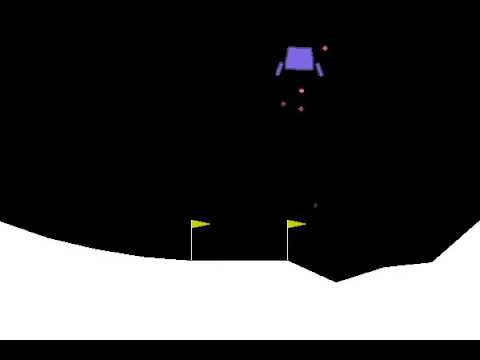
\includegraphics[width=0.4\textwidth]{lunarlander.jpg}
\caption{LunarLander-v2: \url{https://gym.openai.com/envs/LunarLander-v2/} \label{fig:lunarlander-v2}}
\end{figure}
\end{center}

\subsection*{Installation instructions (Linux)}

We've provided Python packages that you may need in \texttt{requirements.txt}. To install these packages using pip and virtualenv, run the following commands:
\begin{quote}
\begin{verbatim}
apt-get install swig
virtualenv env
source env/bin/activate
pip install -U -r requirements.txt
\end{verbatim}
\end{quote}
If your installation is successful, then you should be able to run the provided template code:
\begin{quote}
\begin{verbatim}
python imitation.py
\end{verbatim}
\end{quote}

Note: You will need to install \texttt{swig} and \texttt{box2d} in order to install \texttt{gym[box2d]}, which contains the \texttt{LunarLander-v2} environment. You can install \texttt{box2d} by running
\begin{quote}
\texttt{pip install git+https://github.com/pybox2d/pybox2d}
\end{quote}
If you simply do \texttt{pip install box2d}, you may get an error because the pip package for \texttt{box2d} depends on an older version of \texttt{swig}.\footnote{\url{https://github.com/openai/gym/issues/100}} For additional installation instructions, see \url{https://github.com/openai/gym}.

\newpage
\subsection*{Part 1: Imitating an Expert Trajectory (30pts)}
In this section, you will use function approximation to train an agent to replicate a single trajectory.  The target trajectory is provided in \texttt{trajectory.txt}.  The first 8 columns are features that form the state vector and the last 4 columns correspond to the 4 possible actions that
the agent can take.  There should be a total of 747 rows, each with a state-action pair.  

Your task is to use supervised learning to train a model to learn a policy that replicates the single trajectory as closely as possible.  You cannot use an agent that simply memorizes the state-action pairs since it is not realistic in practice for agents to remember every single interaction.  

Tasks and questions:
\begin{enumerate}
    \item Train a model using supervised learning to predict what action should be taken to replicate the trajectory given an input state.  Evaluate your model with the same initial state as the target trajectory once your model reaches $90\%, 95\%, 99\%, 99.5\%, and 100\%$ accuracy. How well does your model replicate the target trajectory at each of the accuracy points?  Provide a visual comparing the path taken in the target trajectory to the path taken by your learned policy at each accuracy point.  Provide details on the architecture and hyperparameters that you use to train your model.  
    
    \textbf{Note:} In order to feed the same initial state to your model as the one used in the target trajectory, run the environment with seed 39.
    \begin{solution}
    \end{solution}
    \item If your model is not able to match the target trajectory, what can you do to help your model replicate the trajectory exactly?  
    \begin{solution}
    \end{solution}
    \item (Extra Credit): Implement the fix you described in the previous section and show that it helps with trajectory following.
    \begin{solution}
    \end{solution}
    
\end{enumerate}

\subsection*{Part 2: Imitating an Expert Policy (30pts)}

In this section, you will implement behavior cloning using supervised imitation learning from an expert policy, and test on the LunarLander-v2 environment. Please write your code in \texttt{imitation.py}; the template code provided inside is there to give you an idea on how you can structure your code, but is not mandatory to use.

We have provided you with an expert, which you will use to generate training data that you can use with the Keras \texttt{fit} method. The expert model's network architecture is given in \texttt{LunarLander-v2-config.json} and the expert weights in \texttt{LunarLander-v2-weights.h5}. You can load the expert model using the following code snippet:
\begin{quote}
\begin{verbatim}
import keras

model_config_path = 'LunarLander-v2-config.json'
with open(model_config_path, 'r') as f:
    expert = keras.models.model_from_json(f.read())

model_weights_path = 'LunarLander-v2-weights.h5f'
expert.load_weights(model_weights_path)
\end{verbatim}
\end{quote}

Tasks and questions:
\begin{enumerate}
\item Use the provided expert model to generate training datasets consisting of 1, 10, 50, and 100 expert episodes. You will need to collect states and a one-hot encoding of the expert's selected actions.
\item Use each of the datasets to train a cloned behavior using supervised learning. For the cloned model, use the same network architecture provided in \texttt{LunarLander-v2-config.json}. When cloning the behavior, we recommend using the Keras \texttt{fit} method. You should compile the model with cross-entropy as the loss function, Adam as the optimizer, and include `accuracy' as a metric. 

For each cloned model, record the final training accuracy after training for at least 50 epochs. Training accuracy is the fraction of training datapoints where the cloned policy successfully replicates the expert policy. Make sure you include any hyperparameters in your report. 
\begin{solution}
\end{solution}
\item Run the expert policy and each of your cloned models on \texttt{LunarLander-v2}, and record the mean/std of the total reward over 50 episodes. How does the amount of training data affect the cloned policy? How do the cloned policies' performance compare with that of the expert policy?
\begin{solution}
\end{solution}

\item Try to imitate the expert policy without the state features corresponding to $x$ and $y$ velocities.  What accuracy are you able to reach?  Run the cloned policy (without velocity information) on \texttt{LunarLander-v2} and record the mean/std of the total reward over 50 episodes. How does your cloned policy perform?  What are ways to help improve the performance of the cloned policy when the state information is incomplete and results in a non-Markovian environment?
\begin{solution}
\end{solution}
\end{enumerate}


\subsection*{References}

\noindent [1] J Andrew Bagnell. An invitation to imitation. Technical report, DTIC Document, 2015.

\end{document}
